\chapter{Especificación del diseño}\label{chap:design}

\section{Visión general}

Este capítulo tiene como objetivo describir la labor de diseño realizada para desarrollar el proyecto, así como las herramientas que han sido necesarios para su realización. En el siguiente listado se describen los aspectos de diseño que se van a explicar en este capítulo:

\begin{itemize}
	\item \textbf{Diseño de la arquitectura}: descripción del diseño elegido para la arquitectura.
	\item \textbf{Diseño del ``mapeo'' la \acrlong{bd}}: descripción del diseño elegido para el ``mapeo'' de la \acrshort{bd}.
	\item \textbf{Diseño de la aplicación web}: descripción del diseño de la aplicación web.

\end{itemize}

\section{Herramientas utilizadas}

Las herramientas que se han utilizado a la hora de diseñar el proyecto son:

\subsection{Django-extensions, Graph Models}

Graph Models es una herramienta para la generación de grafos del modelo relacional a partir de los ficheros \textit{model.py} donde se especifican las clases que conforman el diseño modelo relacional de la aplicación web. Entre algunas de sus características, permite especificar el nombre de varias aplicaciones para combinarlas en un único modelo, incluir herencias, la exclusión de modelos o columnas y modificar la plantilla con la que renderizar el grafo.

Para este proyecto, solo se ha usado sus capacidades para renderizar los siguientes grafos, sin los cuales no hubiera sido capaz de entender el modelo relacional de \acrshort{labman} y hacer uso de las tablas necesarias para modificar la capa de datos del servidor MOAI y el filtrado de la búsqueda avanzada de proyectos y publicaciones:

\begin{itemize}
	\item Diagrama del modelo relacional completo compuesto por entidades de \acrshort{labman}.
	\item Diagrama del modelo relacional de la entidad publicaciones.
	\item Diagrama del modelo relacional de la entidad proyectos.
	\item Diagrama del modelo relacional para el sistema de ``logs'' de Django.
\end{itemize}

\section{Diseño de la arquitectura}

TODO

\begin{figure}[!htbp]
	\centering
	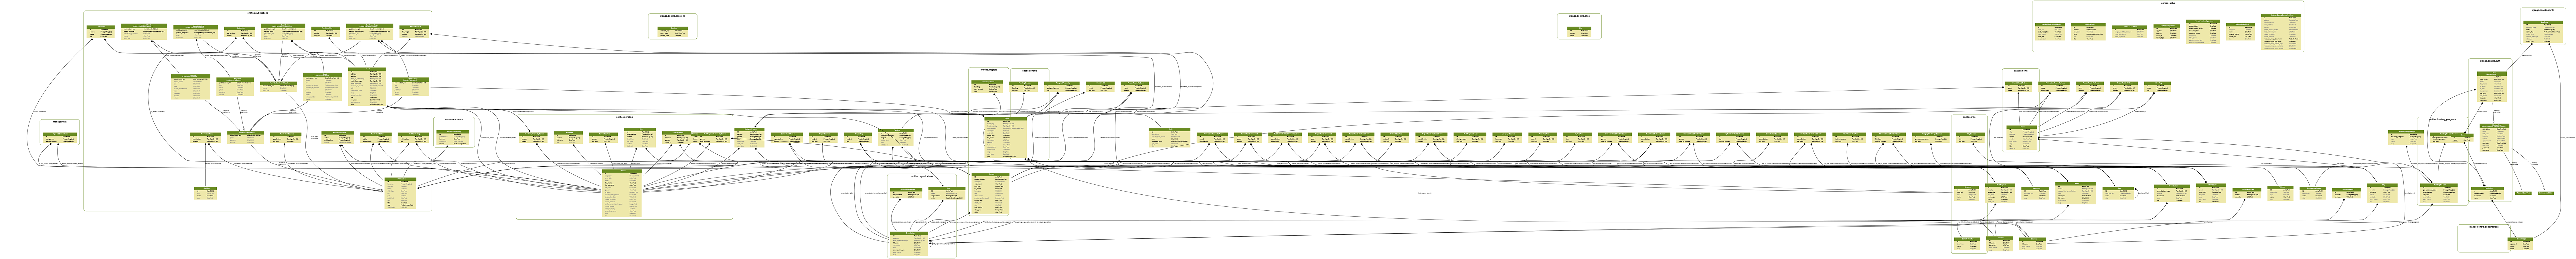
\includegraphics[angle=90, scale=0.072]{fig/dbmodel/labman_model}
	\caption{Modelo de datos relacional completo de \acrshort{labman}}
	\label{fig:labmanmodel}
\end{figure}

\begin{figure}[!htbp]
	\centering
	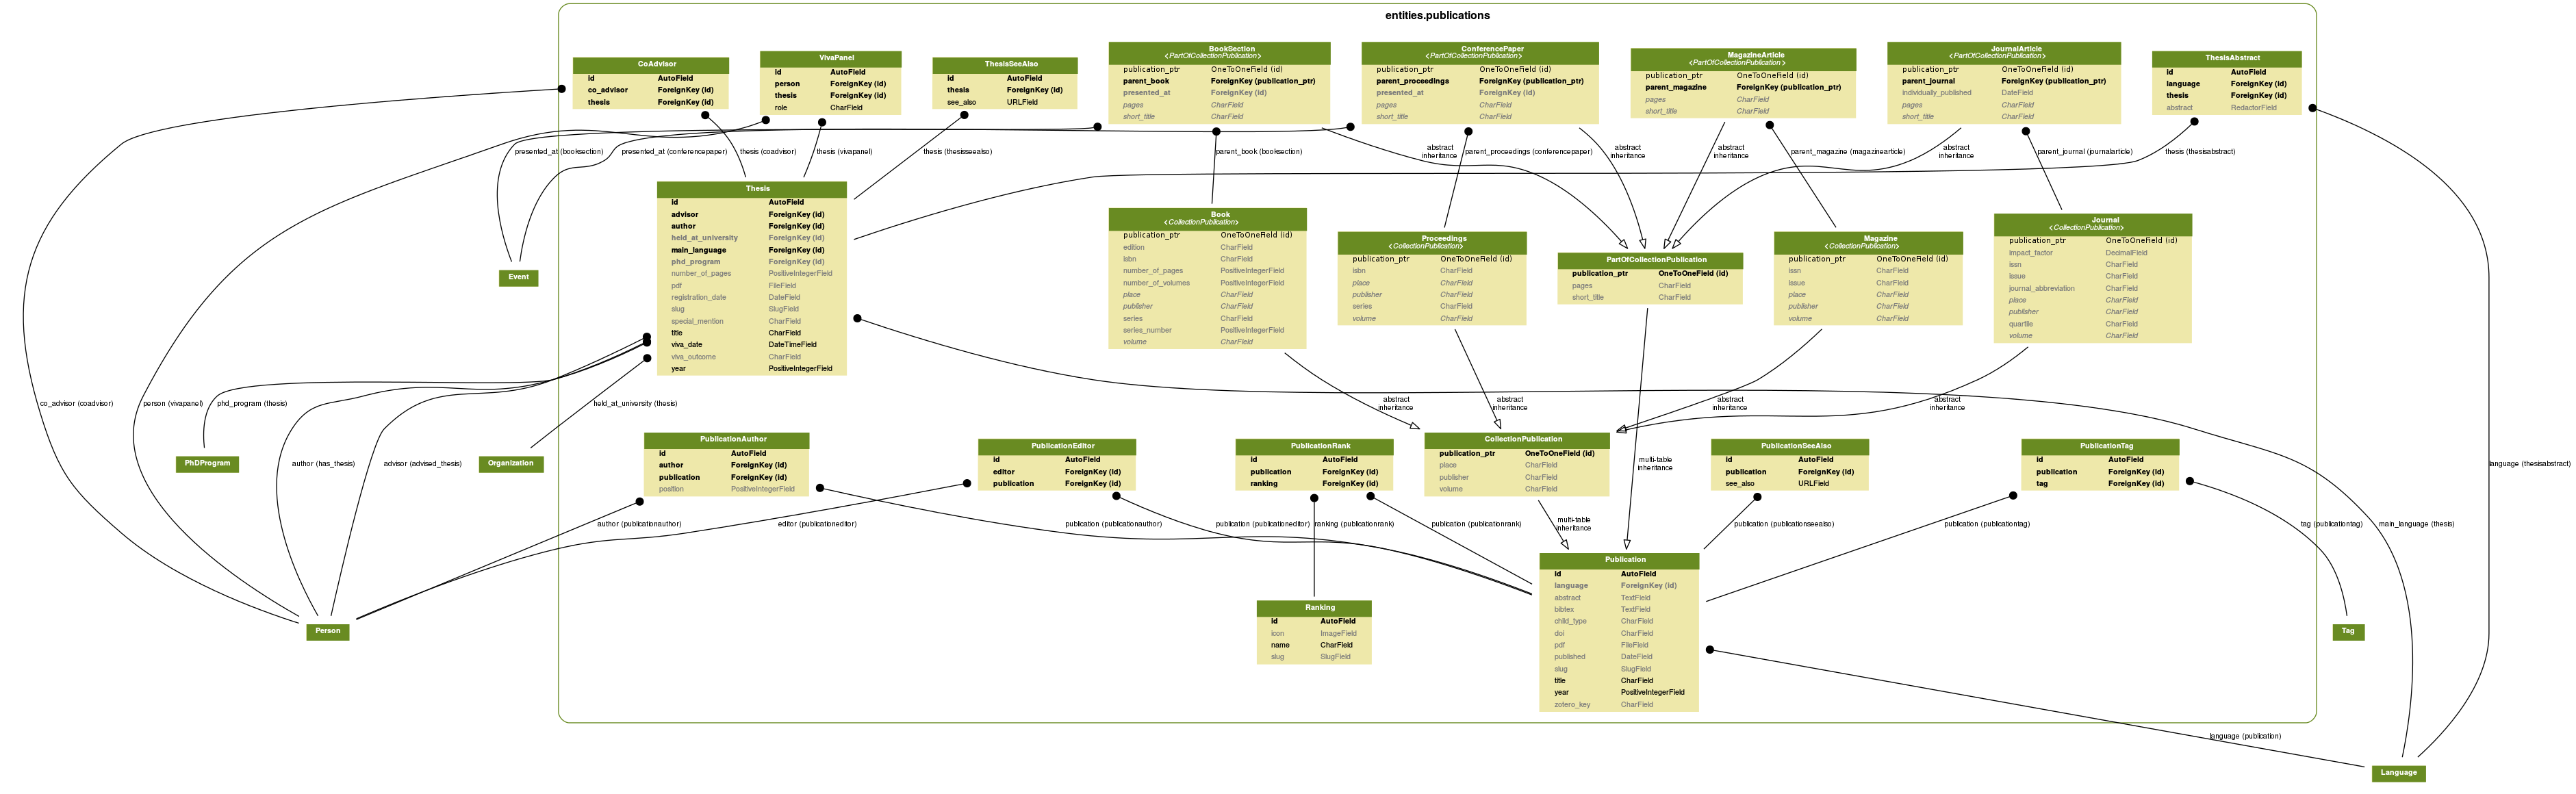
\includegraphics[angle=90, scale=0.17]{fig/dbmodel/publications}
	\caption{Modelo de datos relacional de las publicaciones}
	\label{fig:publicationsmodel}
\end{figure}

\begin{figure}[!htbp]
	\centering
	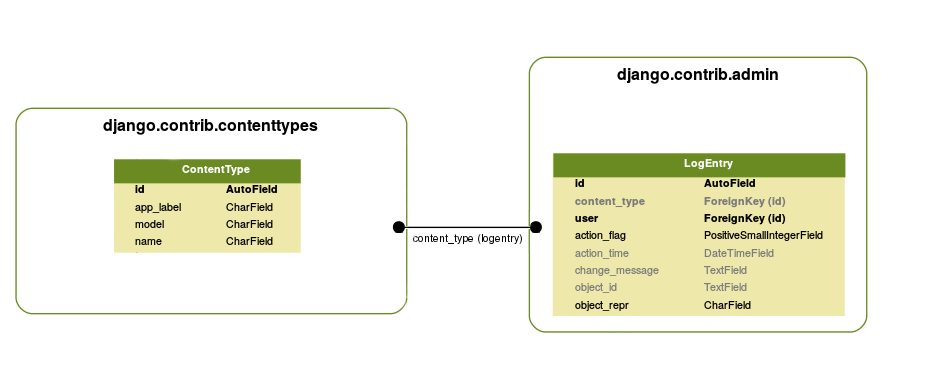
\includegraphics[scale=0.45]{fig/dbmodel/django_log}
	\caption{Modelo de datos relacional del sistema de ``logs'' de Django}
	\label{fig:logsmodel}
\end{figure}

\begin{figure}[!htbp]
	\centering
	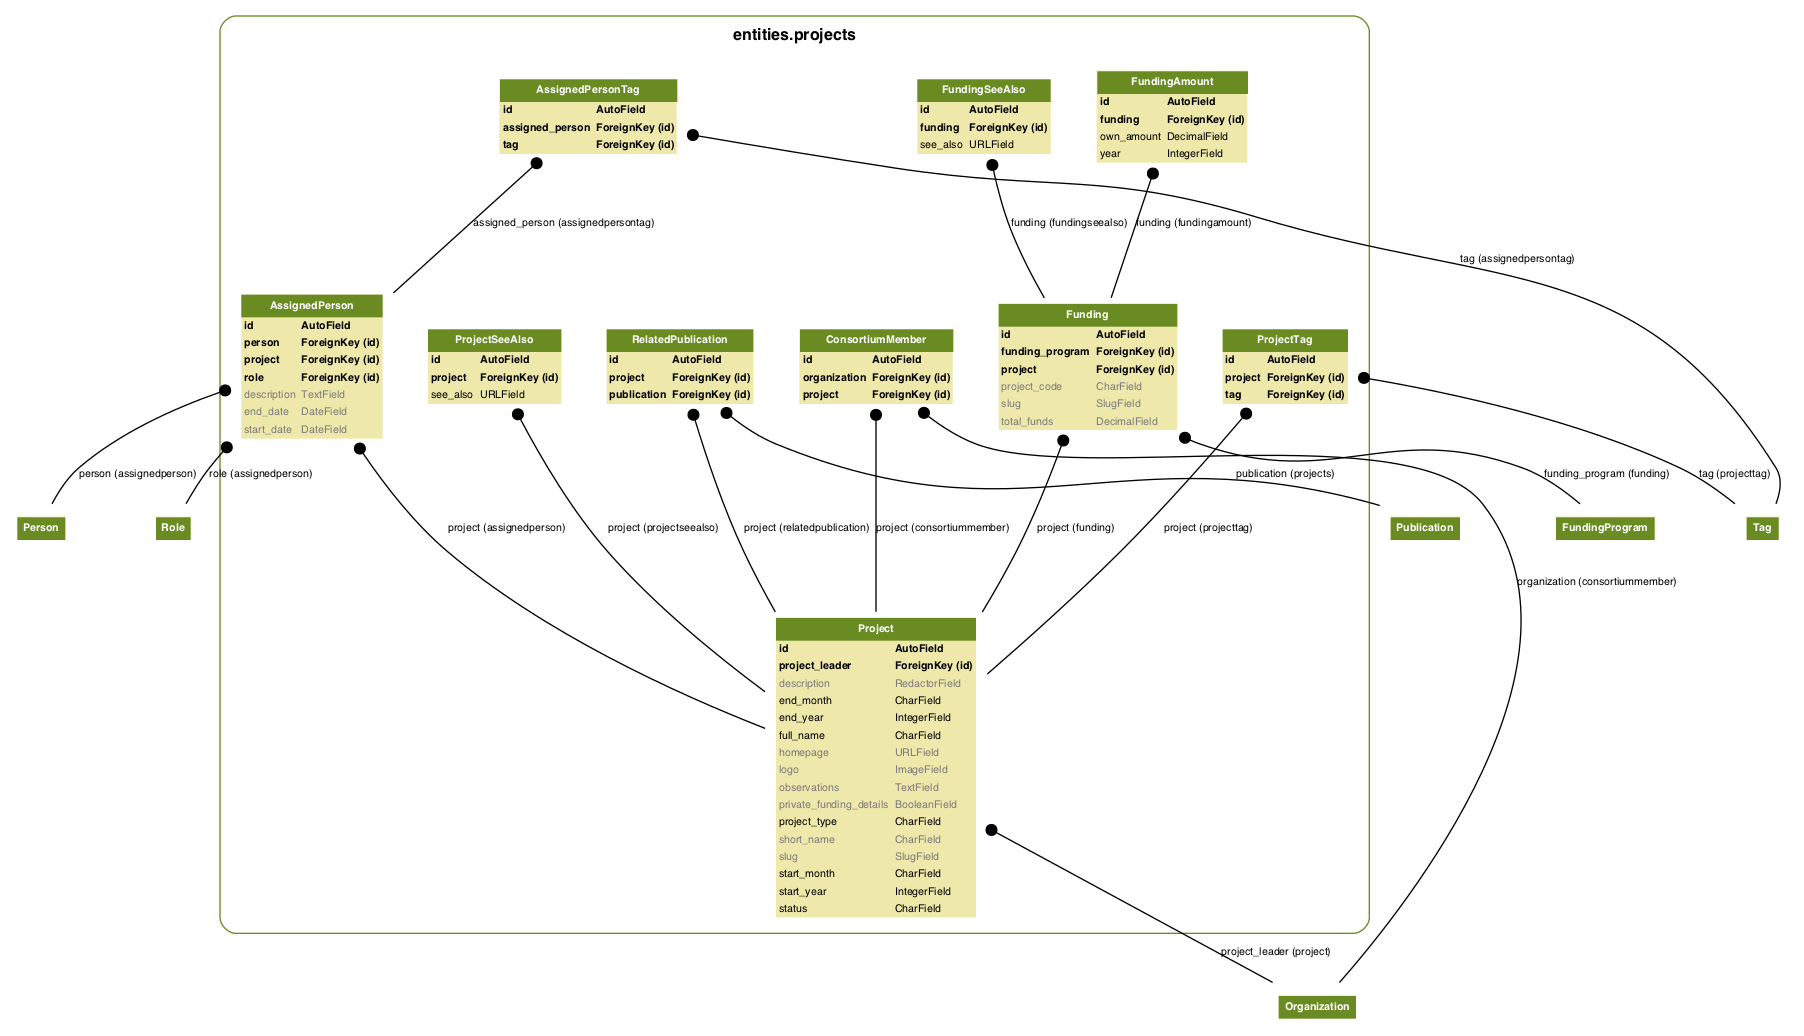
\includegraphics[angle=90, scale=0.35]{fig/dbmodel/projects}
	\caption{Modelo de datos relacional de las proyectos}
	\label{fig:projectsmodel}
\end{figure}
